% ===== INICIO DEL PREÁMBULO =====
\documentclass[oneside,a4paper,linenumbers]{tesina} % version con numeros de linea
%\documentclass[oneside,a4paper]{tesina}            % version sin numeros de linea

% estilo bibliografico
\usepackage{natbib}
\bibliographystyle{apalike}

% A su vez, la clase ya tiene los siguientes paquetes cargados automáticamente, que podrían ser de interés saber para el usuario:
% {color},{hyphenat},{appendix},{lastpage},{babel},{inputenc},{amsmath,amssymb},{ifthen},{graphicx},{caption}
% {setspace},{tabularx},{eqparbox},{ltxcmds},{titletoc},{xcolor},{lineno},{xwatermark}
% Si se quieren agregar más paquetes, se recomienda colocarlos a partir de esta linea y antes de \begin{document}.



% ===== INICIO DEL DOCUMENTO =====
\begin{document}

  \title{Título de la tesina}
  \author{Nombres autor1}{Apellidos autor1}
  \authors{Nombres autor2}{Apellidos autor2}
  \authort{Nombres autor3}{Apellidos autor3}
  \escritura{en} % Se indica que el programa de Posgrado sea "en" o "de" tal área.
  
  \tutor{Dr.Ing.}{Nombres del tutor/a}{Apellidos del tutor/a}{Prof.}
  \cotutor{Dr.Ing.}{Nombres del co tutor/a}{Apellidos del cotutor/a}{(Prof.)}  % Comentar estas líneas si no son necesarias.
  \referenteexterno{Dr.Ing.}{Nombre del referente externo}{Apellido}{(Prof.)}

  \examiner{Dr.Ing.}{Nombre del 1er Examinador}{Apellido}{(Prof.)}
  \examiner{Dr.Ing.}{Nombre del 2do Examinador}{Apellido}{(Prof.)}
  \examiner{Dr.Ing.}{Nombre del 3er Examinador}{Apellido}{(Prof.)}
  
  \graduatename{Nombre de Carrera}
  \institute{Instituto, Facultad }{Sigla}  % La primer institución es la principal.
  
  \graduatelocation{Montevideo}{Uruguay}
  
  \date{28}{11}{2016} % Fecha del documento.

  \keyword{1ra palabra clave}
  \keyword{2da palabra clave}
  \keyword{3ra palabra clave}
  \keyword{4ta palabra clave}
  \keyword{5ta~palabra clave}
  
  \foreignkeyword{1st keyword}
  \foreignkeyword{2nd keyword}
  \foreignkeyword{3rd keyword}
  \foreignkeyword{4th keyword}
  \foreignkeyword{5th keyword}
        
  \maketitle  % Comando que genera el título de la tesis.
  
  \frontmatter  % Comando que genera la portadilla, el catalogo y el tribunal de evaluación. NO COMENTAR
  

  
  \dedication{(Dedicatoria, opcional) A alguien cuyo valor es digno de ella.}


  \chapter*{Agradecimentos}

Quisieramos agredecer a...

  \epigrafe{{\normalfont{(Epígrafe, opcional)}} Frase que alude al tema de trabajo.}{Autor}


  \begin{abstract}

En esta tesis se presenta...

\end{abstract}


  \begin{foreignabstract}

In this work, we present ...

\end{foreignabstract}
  
  \listoffigures	         % Lista de figuras
  \listoftables	         % Lista de tablas
  
  \tableofcontents           % Tabla de contenidos

  \mainmatter % Comando que genera las listas y capítulos. NO COMENTAR
    
  \chapter{Título de capítulo de introducción}

El presente documento establece los aspectos más importantes del formato de las tesinas a realizar en el marco de la Asignatura \textit{Proyecto de Investigación e Innovación en Ingeniería Estructural} de la carrera Ingeniería Civil de la Facultad de Ingeniería de la Universidad de la República. %

Este documento fue generado utilizando una clase de \LaTeX \, llamada \textit{tesinapiiie.cls} la cual fue generada a través de modificaciones en la clase \textit{udelartex.cls}. \footnote{La clase UdelaRTeX fue desarrollada por la Comisión Académica de Posgrado de la Universidad de la República para la realización de tesis de posgrado e implementada por los docentes del IET P. Castrillo y M. Caballero, por más información visitar \url{http://tesis.posgrados.udelar.edu.uy/TallerTesis/UdelaRTeX}.}

El uso de la clase \textit{tesinapiiie} permite a los estudiantes enfocarse en la generación de contenido ya que todo el estilo de la tesina es automáticamente generado por \LaTeX \, así como también se recomienda que la bibliografía sea introducida a través de archivos .bib generados con gestores de bibliografía adecuados. %



\section{Formato del texto, esto es un título de sección}

En el caso de preferir usar otro procesador de textos los estudiantes deberán aplicar el formato definido en este documento. %
%
A continuación se destacan algunos puntos importantes del estilo.

La fuente utilizada para el texto normal es:
\begin{itemize}
	\item \textit{mathptmx} en \LaTeX 
	\item \textit{Times new roman} en MS-Office
	\item \textit{Liberation serif} en LibreOffice
\end{itemize}
%
o equivalentes en otros editores de texto. %
El tamaño de la fuente de texto normal es 12. %
%
El interlineado debe tener un factor de $1.5$. %

En la primer página, el título va en fuente normal tamaño 21 y los logos de las instituciones tienen una altura de 16 mm.

Las versiones de la tesina que vayan a ser revisadas o evaluadas deben tener todas las lineas numeradas como se muestra en este documento. %
%
Estas lineas no deberán estar en la versión final a entregar en biblioteca.

\subsection{Secciones, esto es un título de subsección}


Los títulos de capítulos en negrita y tamaño 24. %
%
Los títulos de las secciones en negrita y tamaño 17.
%
Los títulos de las subsecciones en negrita y tamaño 14.

Los títulos o descripción de las figuras y tablas se escriben en tamaño 11 y usando la negrita como se ve en el ejemplo de la \autoref{tab:comp} .

\subsubsection{Subsubsección}

Los títulos de subsubsecciones van en tamaño 12 y negrita.

\section{Hoja}

La hoja a usar es A4 y los márgenes son 

\begin{itemize}
  \item superior: 3.5cm
  \item inferior: 3cm
  \item izquierdo: 4.0cm
  \item derecho: 3.0cm
\end{itemize}


\section{Estilo de citación y referencias}

Para las referencias bibliográficas se utiliza el estilo definido por la \textit{American Psychology Association} APA \footnote{Ejemplos de la norma se pueden ver en \url{https://owl.english.purdue.edu/media/pdf/20110928111055_949.pdf}}.

Para mostrar ejemplos en la tesina se pueden citar por ejemplo artículos \citep{article-example}, o libros \citep{book-example}, usando el comando \verb|\citep| de \LaTeX \, o también citar al autor utilizando el comando \verb|\cite|, como: \cite{article-example}.

También se pueden citar varios documentos: \citep{Rosati2008,Krour2013,LeMagorou2002}.


 % Se carga el capítulo 01
  \chapter{Ejemplo capítulo} \label{sec2}

\section{Sección}

\subsection{Subsección} \label{subsec}

\subsubsection{Subsubsección}
 % Se carga el capítulo 02
  \chapter{Capítulo}

Ejemplo de referencia a un anexo (Anexo \ref{Ane1}).



 % Se carga el capítulo 03
  \chapter{Ejemplo de capítulo de resultados}


\section{Sección}

Las tablas se pueden referenciar como: en la \autoref{tab:comp} se muestran valores.

\begin{table}[h!]
\centering
\caption{Descripción de tabla.}
\label{tab:comp}
\begin{tabular}{|c|c|c|}
  \hline
  $t$ (seg) & $x$(t) & $y$(t)\\
  \hline
  1 & 0.0000 & 0.0001\\
  2 & 0.5000 & 0.2498\\
  3 & 1.0000 & 1.0000\\
  4 & 1.5000 & 2.2403\\
  5 & 2.0000 & 4.0010\\
  6 & 2.5000 & 6.2459\\
  \hline
\end{tabular}
\end{table}

También se pueden referenciar las figuras como la \autoref{fig:comp}.

\begin{figure}[h!]
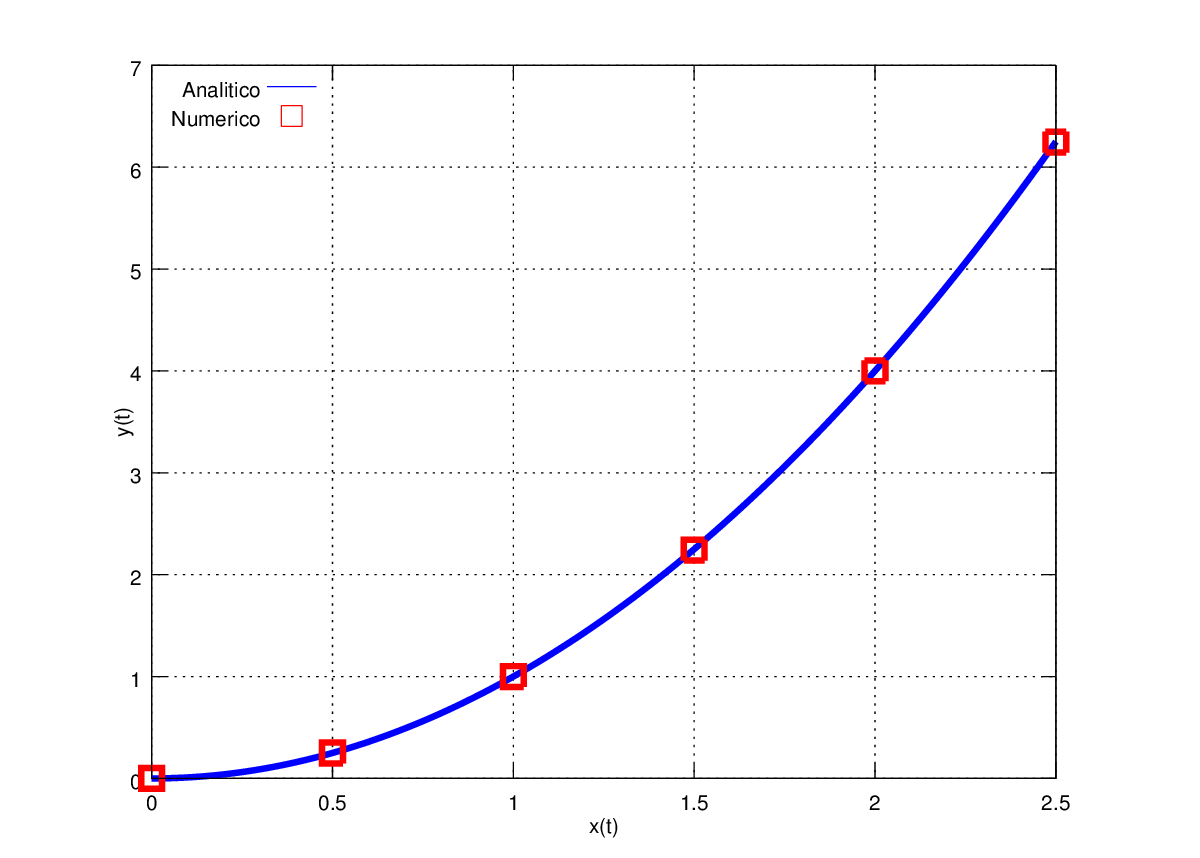
\includegraphics[width=\textwidth]{imagenes/chap4/x_vs_y}
\caption{Descripción de figura, también se deben incluir referencias si la imagen no fue creada por los autores \citep{LeMagorou2002}.}
\label{fig:comp}
\end{figure}

Esto es un ejemplo de ecuación... ver Ecuación~\eqref{eqn:ref}.
\begin{equation}\label{eqn:ref}
\dot{w} = \int_0^T \int_{\Omega} \sigma(t) : \dot{\varepsilon}(t) \, dV \, dt
\end{equation}


También se pueden referenciar otras secciones de la tesina como el \autoref{sec2}, o la \autoref{subsec}, que se encuentra en la página \pageref{sec2}. % Se carga el capítulo 04
  %Seguir copiando la linea de arriba para agregar más capítulos.


  \backmatter % Comando que generalos apéndices, anexos y bibliografía. NO COMENTAR
  
  \bibliography{bibliografia/biblio_1,bibliografia/biblio_2,bibliografia/otros} % Agregar la cantidad de archivos .bib que se tengan para la bibliografía.
  \bibend  
  
  \apenarabicnumbering
  \apenmatter
  \chapter{Título apéndice}


  \chapter{Otro apéndice}\label{Ape2}
Contenido
  
  \anexarabicnumbering
  \anexmatter
  \chapter{Título anexo}\label{Ane1}

Contenido...
  
\end{document}

% ===== FIN DEL DOCUMENTO =====